% \VignetteIndexEntry{survJamda package vignette}

\documentclass[a4paper]{article}
\usepackage{Sweave}
\usepackage{graphicx}
\begin{document}
%%%%%%%%%%%%%%%%%%%%%%%%%%%%%%%%%%%%%%%%%%%%%%%%%
\pagestyle {empty}

\begin{center}
 \LARGE
\textbf{SurvJamda, an R package to predict patients' survival and risk assessment using joint analysis of microarray gene expression data}
\large

\vspace{5cm}
Haleh Yasrebi
\end{center}
%\dosecttoc
\newpage
\pagestyle{plain}
\pagenumbering{roman}
\tableofcontents
\newpage
\pagenumbering{arabic}
\section{Evaluation of gene signatures by cross validation}
The performance of the gene signatures derived from the single or merged data sets can be evaluated in ten iterations of cross validation. To evaluate the performance of a gene signature (100-gene signature by default) derived from a single data set, the following script can be invoked:

\begin{Schunk}
\begin{Sinput}
> data(gse4335)
> data(gse4335pheno)
> iter.crossval(gse4335, gse4335pheno[, 6], gse4335pheno[, 5])
\end{Sinput}
\end{Schunk}

To observe the frequency of the CYB5D1 gene selection (Yasrebi et al. 2009, PLoS
ONE 4(10): e7431, 2009), the following script should be invoked:

\begin{Schunk}
\begin{Sinput}
> iter.crossval(gse4335, gse4335pheno[, 6], gse4335pheno[, 5], 
+     gn.nb = 1, gn.nb.display = 1)
\end{Sinput}
\end{Schunk}

If the \verb+plot.roc+ parameter is set to 1, the ROC curves generated in 10-iterations of cross-validation are displayed. The following figure illustrates the AUC curves of the 1-gene signature derived from the GSE4335 data set:
\begin{Schunk}
\begin{Sinput}
> iter.crossval(gse4335, gse4335pheno[, 6], gse4335pheno[, 5], 
+     plot.roc = 1, gn.nb = 1, gn.nb.display = 1)
\end{Sinput}
\end{Schunk}

\begin{figure}[h]
\begin{center}
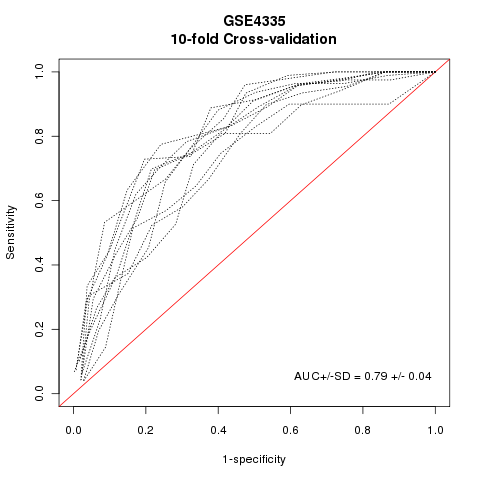
\includegraphics[scale = 0.5]{AUC10fCVgse43351gn.png}
\end{center}
\end{figure}

The same function \verb+iter.crossval+ can be used to assess the performance of the gene signatures derived from the merged data sets adjusted by Z-score normalization:

\begin{Schunk}
\begin{Sinput}
> data(gse4335)
> data(gse4335pheno)
> data(gse1992)
> data(gse1992pheno)
> common.gene = intersect(colnames(gse4335), colnames(gse1992))
> data = rbind(gse4335[, common.gene], gse1992[, common.gene])
> surv = c(gse4335pheno[, 6], gse1992pheno[, 19])
> censor = c(gse4335pheno[, 5], gse1992pheno[, 18])
> iter.crossval(data, surv, censor, zscore = 1)
\end{Sinput}
\end{Schunk}

The \verb+iter.crossval.combat+ function is used to evaluate the performance of the gene signatures derived from the merged data sets adjusted by ComBat:

\begin{Schunk}
\begin{Sinput}
> data(gse4335)
> data(gse4335pheno)
> data(gse1992)
> data(gse1992pheno)
> common.gene = intersect(colnames(gse4335), colnames(gse1992))
> data = rbind(gse4335[, common.gene], gse1992[, common.gene])
> surv = c(gse4335pheno[, 6], gse1992pheno[, 19])
> censor = c(gse4335pheno[, 5], gse1992pheno[, 18])
> batchID = rep(1, nrow(gse4335))
> batchID = c(batchID, rep(2, nrow(gse1992)))
> iter.crossval.combat(data, surv, censor, batchID)
\end{Sinput}
\end{Schunk}
\section{Evaluation of gene signatures by independent validation}
\subsection{Pair-wise manner}
The performance of a gene signature derived from one data set can be assessed on an independent data set. This process is performed by independent validation in a pair-wise manner and is iterated until all data sets are used as the training and testing sets.

\begin{Schunk}
\begin{Sinput}
> data(gse4335)
> data(gse3143)
> data(gse1992)
> data(gse4335pheno)
> data(gse3143pheno)
> data(gse1992pheno)
> geno.files = c("gse4335", "gse3143", "gse1992")
> surv.data = list(c(gse4335pheno[, 6], gse3143pheno[, 4], gse1992pheno[, 
+     19]), c(gse4335pheno[, 5], gse3143pheno[, 3], gse1992pheno[, 
+     18]))
> main.single.indep.valid(geno.files, surv.data)
\end{Sinput}
\end{Schunk}
\subsection{Leave-one-dataset-out}
The performance of a gene signature derived from a merged data set can be assessed on an independent single data set. This process is referred to as leave-one-dataset-out and is iterated until all data sets are used as the training and testing sets.
\begin{Schunk}
\begin{Sinput}
> data(gse4335)
> data(gse3143)
> data(gse1992)
> data(gse4335pheno)
> data(gse3143pheno)
> data(gse1992pheno)
> geno.files = c("gse4335", "gse3143", "gse1992")
> surv.data = list(c(gse4335pheno[, 6], gse3143pheno[, 4], gse1992pheno[, 
+     19]), c(gse4335pheno[, 5], gse3143pheno[, 3], gse1992pheno[, 
+     18]))
> main.merge.indep.valid(geno.files, surv.data)
\end{Sinput}
\end{Schunk}
To plot ROC curves generated in leave-one-dataset-out based on different time points, \verb+pred.time.indep.valid+ can be invoked as follows:
\begin{Schunk}
\begin{Sinput}
> pred.time.indep.valid(geno.files, surv.data)
\end{Sinput}
\end{Schunk}
\begin{figure}[h]
\begin{center}
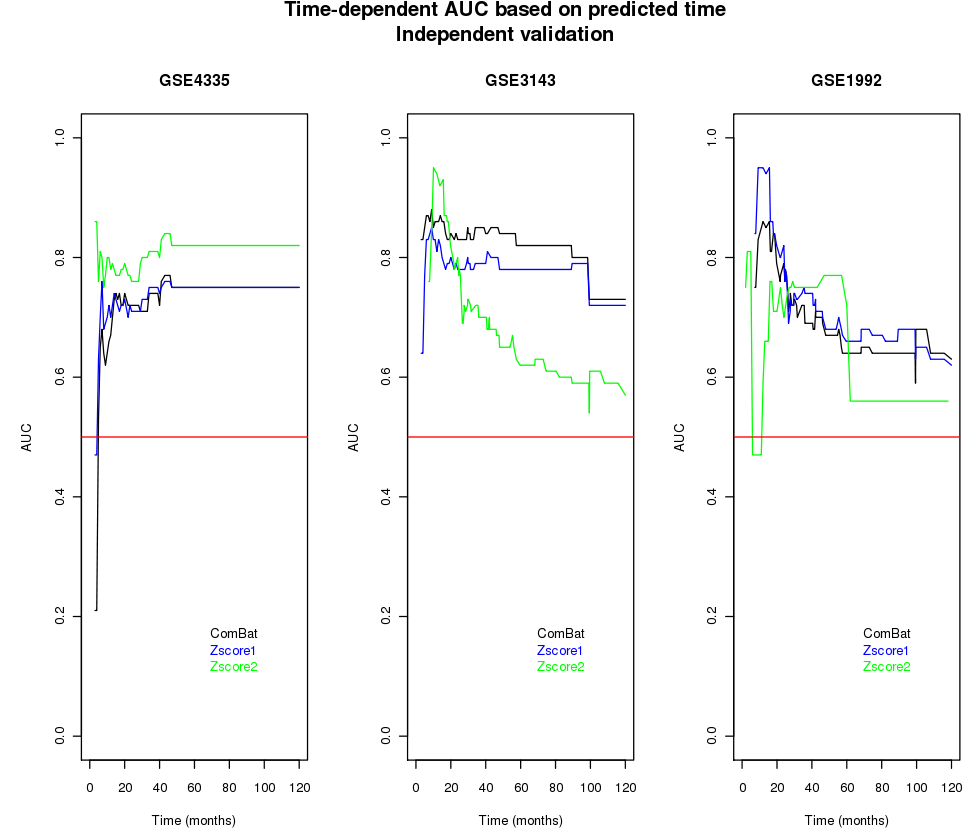
\includegraphics{predictTime.png}
\end{center}
\end{figure}
\section{Evaluation of gene signatures by meta-analysis}
The \verb+meta.main+ evaluates the performance of the gene signatures by meta analysis.
\begin{Schunk}
\begin{Sinput}
> data(gse4335)
> data(gse3143)
> data(gse1992)
> data(gse4335pheno)
> data(gse3143pheno)
> data(gse1992pheno)
> geno.files = c("gse4335", "gse3143", "gse1992")
> surv.data = list(c(gse4335pheno[, 6], gse3143pheno[, 4], gse1992pheno[, 
+     19]), c(gse4335pheno[, 5], gse3143pheno[, 3], gse1992pheno[, 
+     18]))
> meta.main(geno.files, surv.data)
\end{Sinput}
\end{Schunk}
\section{Evaluation of gene signatures by simulation}
Survival data can be simulated using a Weibull distribution to determine if the prediction performance derived from the merged data set is mediated by the correlation among the genes.
\begin{Schunk}
\begin{Sinput}
> proc.simulate()
\end{Sinput}
\end{Schunk}
\section{Evaluation of gene signatures by subsetting a data set}
A data set can be split to different subsets to determine if the performance derived from its subsets
is improved by the increase of sample size. Each subset can then be split 100 times into the independent
training and testing sets. The sample size of the training set is set by the user (20,50,...,up
to 2/3 of the complete set) and the remaining samples are used for the testing set. A gene signature
will be derived from the training set and assessed on the testing set.

The performance obtained from the larger subsets and ultimately, the complete set is more likely
higher than the performance generated from the smaller subsets. If it is not the case, the performance
improvement might have been retained by factors such as heterogeneity with respect to patient cohorts or tumor characteristics.

\begin{Schunk}
\begin{Sinput}
> data(gse4335)
> data(gse4335pheno)
> iter.subset(gse4335, gse4335pheno[, 6], gse4335pheno[, 5])
\end{Sinput}
\end{Schunk}
\end{document}
